
\item A device (Fig. 1.26) consists of a smooth L-shaped rod located in a horizontal plane and a sleeve \( A \) of mass \( m \) attached by a weightless spring to a point \( B \). The spring stiffness is equal to \( \kappa \). The whole system rotates with a constant angular velocity \( \omega \) about a vertical axis passing through the point \( O \). Find the elongation of the spring. How is the result affected by the rotation direction?
    \begin{center}
        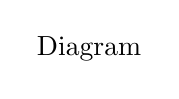
\begin{tikzpicture}
            \node at (0, 0) {Diagram};
        \end{tikzpicture}
    \end{center}

\begin{solution}
    \begin{center}
        \begin{tikzpicture}
            \pic at (0, 0) {frame=3cm};
        \end{tikzpicture}
    \end{center}
    
    \begin{align*}
        \intertext{From $F_n = mw_n$}
        N \sin \theta + F \cos \theta &= m \omega^2 r \tag{1} 
        \intertext{where \( r \cos \theta = (l_0 + \Delta l) \).}
        \intertext{Similarly, from \( F_t = mw_t \)}
        N \cos \theta - F \sin \theta &= 0 \quad \text{or} \quad N = F \sin \theta / \cos \theta \tag{2} 
        \intertext{From Eqs. (1) and (2)}
        F (\sin \theta / \cos \theta) \cdot \sin \theta + F \cos \theta &= m \omega^2 r \\
        &= m \omega^2 (l_0 + \Delta l)/ \cos \theta \\
        \intertext{On putting \( F = \kappa \Delta l \)}
        \kappa \Delta l \sin^2 \theta + \kappa \Delta l \cos^2 \theta &= m \omega^2 (l_0 + \Delta l) \\
        \intertext{On solving, we get}
        \Delta l &= \dfrac{ m \omega^2 - l_0}{\kappa -m \omega^2} = \dfrac{ l_0}{(\kappa/ m\omega^2 -1)}
        \intertext{It is independent of the direction of rotation.}
    \end{align*}
\end{solution}
